\section{Auswertung}
\label{sec:Auswertung}
\subsection{a) Bestimmung der Zeitkonstanten RC}
Zur Bestimmung der Zeitkonstanten RC werden aus der Entladekurve in \ref{fig:plotrc} die Werte für $U_\text{C}$ abgelesen.
$U_\text{0}$ wurde bestimmt zu $U_\text{0}=\SI{7.28}{\ohm} $.
Durch Umformung wird Formel \eqref{eqn:aufladung} zu
\begin{equation}
\label{eqn:ausgleich1}
\ln{\frac{U_\text{C}}{U_\text{0}}}=-\frac{1}{RC}t .
\end{equation}
Zur Bestimmung wird nun $\ln{\frac{U_\text{C}}{U_\text{0}}}$ gegen die Zeit $t$ aufgetragen.
Aus der Steigung der Regressionsgeraden nach Gleichung \eqref{eqn:ausgleich1} ergibt sich nun die berechnete Zeitkonstante zu
\begin{equation*}
  \centering
  RC = (0.48 \pm 0.03) \cdot 10^{-3} \si{\second}
\end{equation*}
\begin{table}
\begin{tabular}{ccc}
$U_\text{C}$/$\si{\volt}$ & $\ln{(\frac{U_\text{C}}{U_\text{0}})}$ & $t$ /$10^{-6}\si{\second}$ \\
6.04 & -0.186726850262 & 0.0 \\
4.04 & -0.588886170236 & 0.25 \\
2.76 & -0.96990018248 & 0.5 \\
1.8 & -1.39734419731 & 0.75 \\
1.08 & -1.90816982107 & 1.0 \\
0.56 & -2.56494935746 & 1.25 \\
0.24 & -3.41224721785 & 1.5 \\
\end{tabular}
\end{table}

\begin{figure}
	\centering
	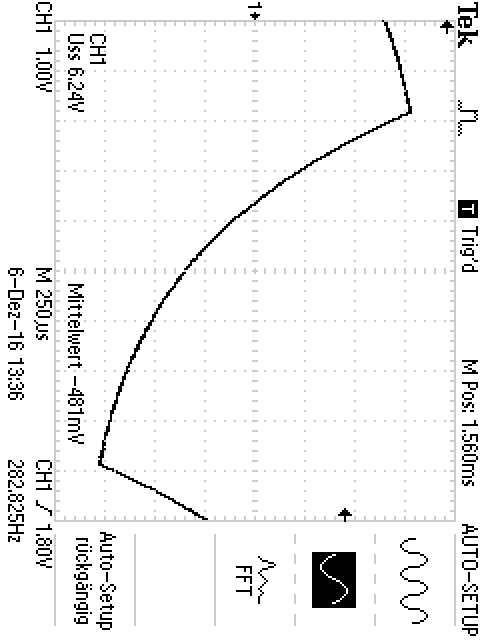
\includegraphics[angle=90]{bilder/F0000TEK.JPG}
	\caption{Aufgabenteil a: Bestimmung der Zeitkonstante $RC$}
	\label{fig:plotrc}
\end{figure}

\begin{figure}
  \centering
  \includegraphics{build/test.pdf}
  \caption{Lineare Regression zur Bestimmung der Zeitkonstanten $RC$}
  \label{fig:plota}
\end{figure}


\begin{figure}
  \centering
  \includegraphics{build/amplitude.pdf}
  \caption{Regression zur Bestimmung der Zeitkonstanten $RC$}
  \label{fig:plota}
\end{figure}
\begin{table}
  \centering

\begin{tabular}{cc}
  \toprule
$U$/ $10^{-3} \si{\volt}$ & $\omega$/$\si{\Hz}$ \\
\midrule
280.0 & 4.24 \\
440.0 & 10.0 \\
488.0 & 15.0 \\
504.0 & 20.0 \\
520.0 & 35.0 \\
512.0 & 60.0 \\
488.0 & 90.0 \\
432.0 & 150.0 \\
360.0 & 230.0 \\
288.0 & 320.0 \\
208.0 & 500.0 \\
112.0 & 1000.0 \\
68.0 & 2000.0 \\
23.0 & 5000.0 \\
12.0 & 10000.0 \\
\bottomrule
\end{tabular}
\end{table}

\subsection{d) Integration}

\begin{figure}
	\centering
	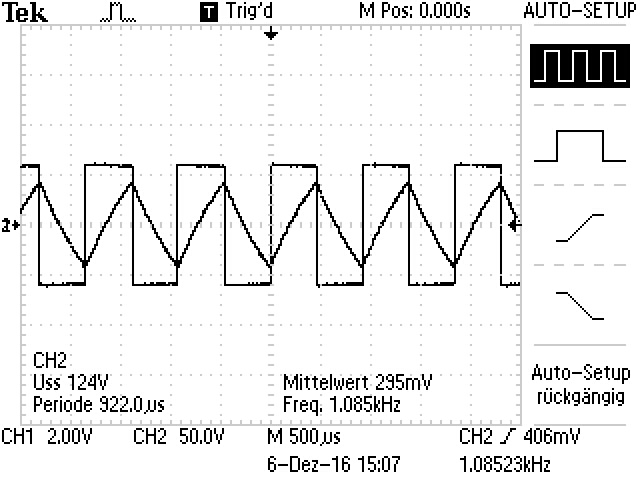
\includegraphics[width=0.75\textwidth]{bilder/ALL0001/F0001TEK.JPG}
	\caption{Aufgabenteil d: Rechteckspannung}
	\label{fig:rechteck}
\end{figure}

In Abbildung \ref{fig:rechteck} ist die Rechteckspannung sowie die über das RC-Glied integrierte Rechteckspannung dargestellt.
Die integrierte Rechteckspannung ist wie zu erwarten eine Dreiecksspannung.


\begin{figure}
	\centering
	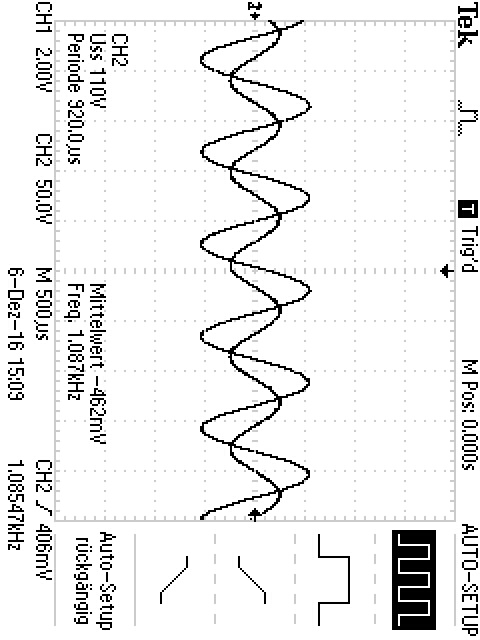
\includegraphics[width=0.75\textwidth]{bilder/ALL0002/F0002TEK.JPG}
	\caption{Aufgabenteil d: Sinusspannung}
	\label{fig:sinus}
\end{figure}

Der Spannungsverlauf der Sinusspannung ist in Abbildung \ref{fig:sinus} dargestellt. Wie zuvor ist die Kosinusspannung - integrierte Sinusspannung - außerdem in diesem Plot aufgezeichnet.


\begin{figure}
	\centering
	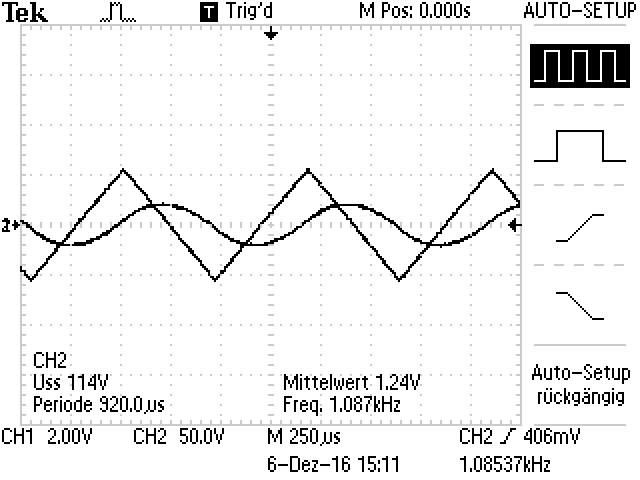
\includegraphics[width=0.75\textwidth]{bilder/ALL0003/F0003TEK.JPG}
	\caption{Aufgabenteil d: Dreiecksspannung}
	\label{fig:dreieck}
\end{figure}

In Abbildung \ref{fig:dreieck} ist Dreieck und Parabelspannung zu sehen
